%% Простая презентация с примером включения программного кода и
%% пошаговых спецэффектов
\documentclass{beamer}
\usepackage{fontspec}
\usepackage{xunicode}
\usepackage{xltxtra}
\usepackage{xecyr}
\usepackage{hyperref}
\setmainfont[Mapping=tex-text]{DejaVu Serif}
\setsansfont[Mapping=tex-text]{DejaVu Sans}
\setmonofont[Mapping=tex-text]{DejaVu Sans Mono}
\usepackage{polyglossia}
\setdefaultlanguage{russian}
\usepackage{graphicx}
\usepackage{listings}
\lstdefinestyle{mycode}{
  belowcaptionskip=1\baselineskip,
  breaklines=true,
  xleftmargin=\parindent,
  showstringspaces=false,
  basicstyle=\footnotesize\ttfamily,
  keywordstyle=\bfseries,
  commentstyle=\itshape\color{gray!40!black},
  stringstyle=\color{red},
  numbers=left,
  numbersep=5pt,
  numberstyle=\tiny\color{gray},
}
\lstset{escapechar=@,style=mycode}


% счетчик слайдов
\addtobeamertemplate{navigation symbols}{}{%
    \usebeamerfont{footline}%
    \usebeamercolor[fg]{footline}%
    \hspace{1em}%
    \insertframenumber/\inserttotalframenumber
}
\usepackage{graphicx}       % работа с картинками
\usepackage[export]{adjustbox}  % еще про место картинки (width,right/left])
\usepackage{multicol,caption,float, subfig} % картинки

\usepackage{multirow} % для няшных табличек      


\begin{document}
\title{Рекомендательная систета для образовательного контента}
\subtitle{бакалаврская работа}
\author{Волжина Елена\\{\footnotesize\textcolor{gray}{группа 441\\руководитель А.С. Ярыгина}}}
\institute{СПбГУ}
\date{1 июня 2016г.}
\frame{\titlepage}

\begin{frame}\frametitle{Введение}
% в современном мире онлайн-образование имеет большую популярность, т.к. ...
% ниже можно увидеть статистику
% по сравнению с офлайн-образованием онлайн имеет множество плюсов, но также есть и минусы. один из них -- отсутствие прямой связи между преподавателем и студентом. вследствие этого оказывается востребована рекомендательная система, которая может подсказать пользователю, что ему можно изучить по интересным ему темам, предложить что-то новое, а также помочь в освоении материала в удобном ему темпе и формате, бесплатно без смс
\begin{itemize}
\item онлайн-образование
    \begin{table}[t]
        \caption{Платформы с онлайн-курсами}
        \begin{center}
        \begin{tabular}{c|c|c}
        \hline
        Название & Год запуска & Пользователей \\
        \hline
        \hline
        Coursera & 2012 & 15 млн \\
        edX & 2012 & 5 млн \\
        Udacity & 2012 & 1.6 млн \\
        Stepic.org & 2013 & 200 тыс. \\
        \hline
        \end{tabular}
        \end{center}
    \end{table}

\bigskip
\item рекомендательные системы\cite{rec_sys_handbook}
    \begin{itemize}
        \item фильтрация контента
        \item коллаборативная фильтрация
        \item гибридные системы
    \end{itemize}
\end{itemize}
\end{frame}



\begin{frame}\frametitle{Постановка задачи}

\begin{columns}
    \column{0.48\linewidth}
        \begin{itemize}
            \item платформа Stepic.org
            \smallskip
            \item гибридная рекомендательная система
            \bigskip
            \item виды рекомендаций:
                \begin{itemize}
                    \item простые 
                    \item контекстные 
                    \item адаптивные 
                \end{itemize}
        \end{itemize}
    \column{0.48\linewidth}
      \centering
      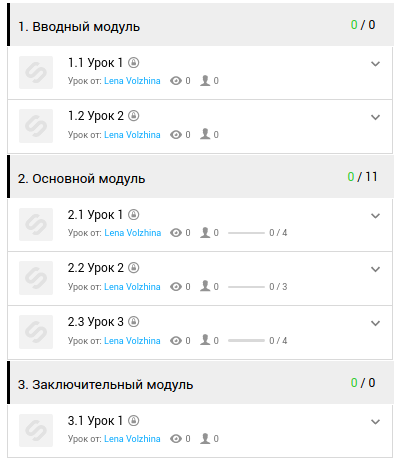
\includegraphics[width=\textwidth]{images/course_structure_shrinked.png}
 \end{columns} 
    
\end{frame}

\begin{frame}\frametitle{Рекомендательная система: хендлеры}
\bigskip
Хендлер: $(user\_data) \rightarrow [(lesson, weight)]$

    \begin{itemize}
        \item LessonsByInterestingTagsHandler
        \item NotFinishedLessonsHandler
        \item TopLessonsHandler
        \item ...
    \end{itemize}

\begin{figure}[H]
    \center{\includegraphics[width=\linewidth]{images/handlers_scheme.png}}
\end{figure}

\end{frame}

\begin{frame}\frametitle{Адаптивные рекомендации: \\MathsGarden}

    \bigskip
    MathsGarden.com\cite{mathsgarden}
    
    \begin{itemize}
        \item Elo chess rating
        \item Item Response theory
        \item High speed, high stakes
    \end{itemize}
    
    \begin{figure}[t]
      \centering
      \subfloat[начальный экран]{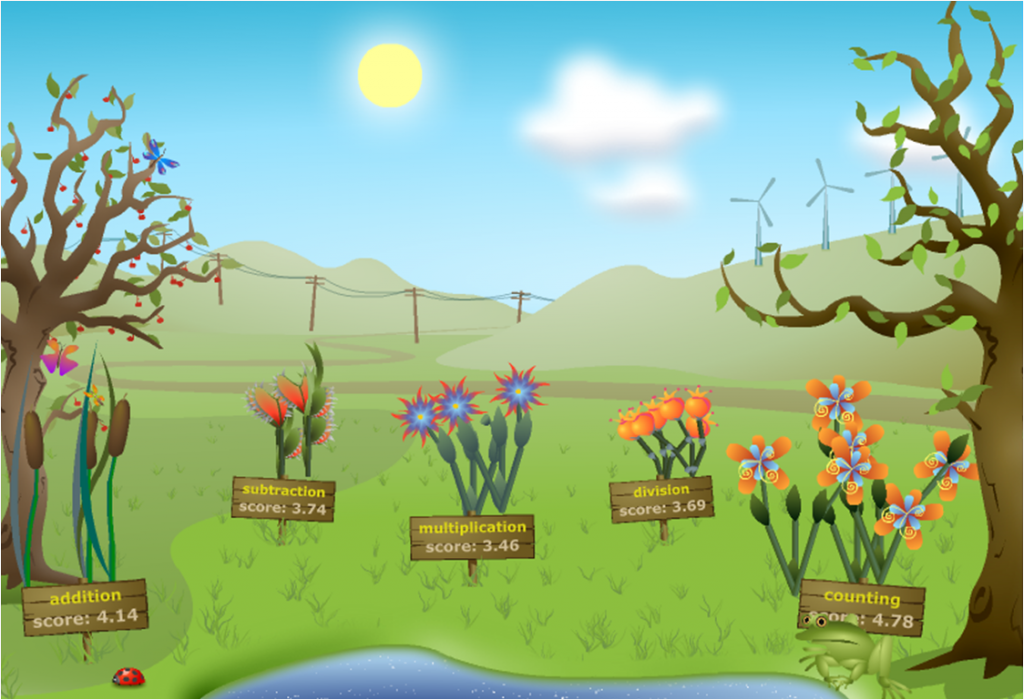
\includegraphics[width=0.4\textwidth]{images/mathsgarden.png} \label{fig_mathsgarden1}}
      \hfill
      \subfloat[решение задачи]{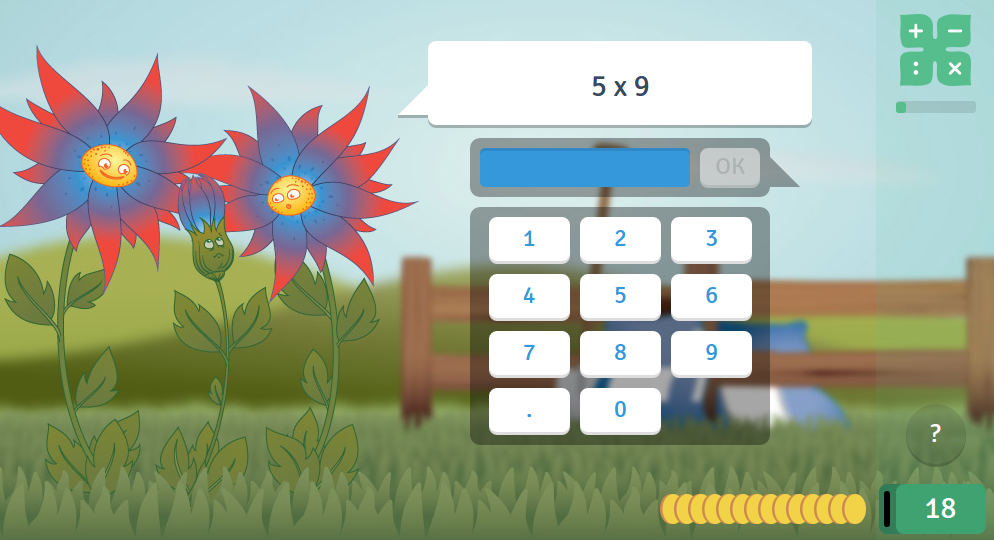
\includegraphics[width=0.5\textwidth]{images/mathsgarden_quiz.png} \label{fig_mathsgarden2}}
      
    \end{figure}
    
\end{frame}


\begin{frame}\frametitle{Адаптивные рекомендации: \\подсчет сложности}
       Elo chess rating
       \medskip
       \begin{itemize}
            \item Арпад Эло, 1978\cite{elo1978rating}
            \medskip
            \item $E(S_j) = \frac{1}{1 + 10 ^ {(\theta_j - \theta_k) / 400}}$, \\где $\theta_j$ и $\theta_k$ -- рейтинги игроков, $S_j \in \{0, 0.5, 1\}$
            \medskip
            \item $\hat{\theta_j} = \theta_j + K(S_j - E(S_j))$
            \medskip
            \item Марк Гликман, 1995: пусть $K$ -- не const \cite{glickman95}
      \end{itemize}
\end{frame}



\begin{frame}\frametitle{Результаты: обычные рекомендации}
\bigskip

\begin{table}[H]
    \begin{tabular}{| c || r| }
      Метрика & Значение \\
      \hline		
      Число сессий & 381868 \\
      Число сессий с реакцией & 18066 \\
      Процент сессий с реакцией &  4.7\% \\
      Число открытых рекомендаций (из 20) & 1.6 \\
      Пройденная часть урока & 0.52 \\
      Число отказов от рекомендации & 184 \\\hline
    \end{tabular}
\end{table}


\begin{figure}[H]
  \centering
  \subfloat[открыто ссылок]{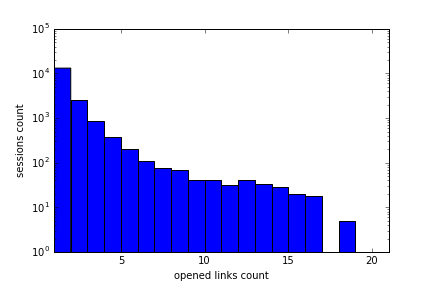
\includegraphics[width=0.4\textwidth]{images/home_page_opened_links_number_hist.png}}
  \hfill
  \subfloat[решено от задачи]{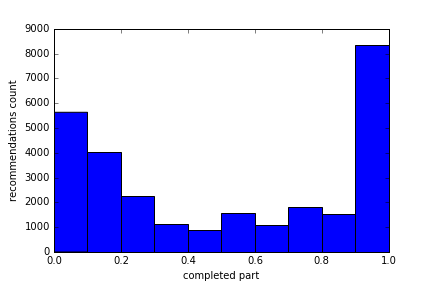
\includegraphics[width=0.4\textwidth]{images/home_page_completed_part_hist.png}}
\end{figure}

\end{frame}


\begin{frame}\frametitle{Результаты: контекстные рекомендации}

\bigskip

\begin{table}[H]
    \begin{tabular}{| c || r| }
      Метрика & Значение \\
      \hline		
      Число сессий & 26995 \\
      Число сессий с реакцией & 15125 \\
      Процент сессий с реакцией &  56\% \\
      Число открытых рекомендаций (из 5) & 1.48 \\
      Пройденная часть урока & 0.5 \\
      Число отказов от рекомендации & 0 \\
      \hline  
    \end{tabular}
\end{table}

\begin{figure}[H]
  \centering
  \subfloat[открыто ссылок]{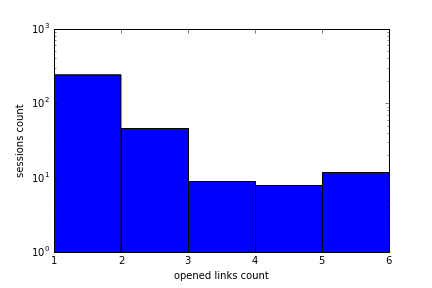
\includegraphics[width=0.4\textwidth]{images/context_opened_links_number_hist.png}}
  \hfill
  \subfloat[решено от задачи]{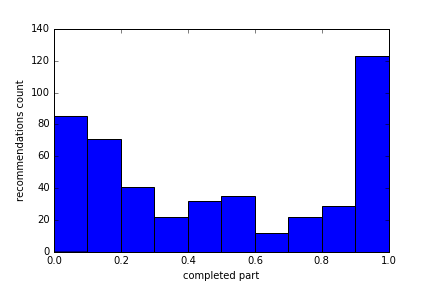
\includegraphics[width=0.4\textwidth]{images/context_completed_part_hist.png}}
\end{figure}

\end{frame}


\begin{frame}\frametitle{Результаты: адаптивные рекомендации}

\begin{table}[H]
    \begin{tabular}{| c || r| }
      Метрика & Значение \\
      \hline		
      Число сессий & 1511 \\
      Число пользователей & 246 \\
      Реакций "решено" & 1329 \\
      Реакций "слишком просто" & 95 \\ 
      Реакций "слишком сложно" & 87 \\
      MSE предсказания исхода & 0.22 \\
      
     \hline  
    \end{tabular}
\end{table}

% Также было исследовано, действительно ли ошибка предсказания для конкретного пользователя или задачи уменьшается со временем. Для этого ошибки были усреднены по пользователям (рисунок \ref{fig:adapt1}) и по задачам (рисунок \ref{fig:adapt2}). На получившихся графиках наблюдается явное, хоть и не равномерное, убывание ошибки.


\begin{figure}[H]
  \centering
  \subfloat[пересчет знаний пользователя]{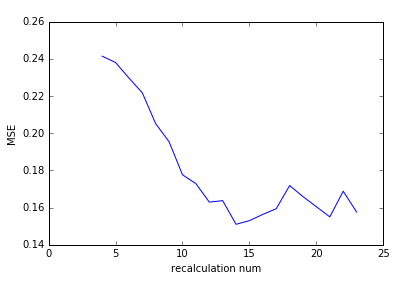
\includegraphics[width=0.45\textwidth]{images/mse_user_skill.png}}
  \hfill
  \subfloat[пересчет сложности задачи]{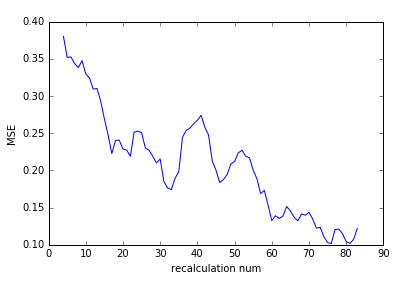
\includegraphics[width=0.45\textwidth]{images/mse_quiz_difficulty.png}}
\end{figure}

\end{frame}


\begin{frame}\frametitle{Планы}
    \begin{itemize}
        \item Развитие адаптивной системы:
            \begin{itemize}
                \item связи между материалами, темами
                \item дискриминативность и другие характеристики задач
            \end{itemize}
        \bigskip
        \item Более глубокий анализ накопленных данных
    \end{itemize}

\end{frame}



\begin{frame}\frametitle{Литература}
\setmonofont[Mapping=tex-text]{CMU Typewriter Text}
\bibliographystyle{plain}  %ieeetr
\bibliography{diploma.bib}
\end{frame}


\begin{frame}
\huge{Спасибо! \\\indent \\\indent Вопросы?}
\end{frame}


\end{document}